\documentclass[]{article}
\usepackage{lmodern}
\usepackage{amssymb,amsmath}
\usepackage{ifxetex,ifluatex}
\usepackage{fixltx2e} % provides \textsubscript
\ifnum 0\ifxetex 1\fi\ifluatex 1\fi=0 % if pdftex
  \usepackage[T1]{fontenc}
  \usepackage[utf8]{inputenc}
\else % if luatex or xelatex
  \ifxetex
    \usepackage{mathspec}
    \usepackage{xltxtra,xunicode}
  \else
    \usepackage{fontspec}
  \fi
  \defaultfontfeatures{Mapping=tex-text,Scale=MatchLowercase}
  \newcommand{\euro}{€}
\fi
% use upquote if available, for straight quotes in verbatim environments
\IfFileExists{upquote.sty}{\usepackage{upquote}}{}
% use microtype if available
\IfFileExists{microtype.sty}{%
\usepackage{microtype}
\UseMicrotypeSet[protrusion]{basicmath} % disable protrusion for tt fonts
}{}
\usepackage[margin=1in]{geometry}
\usepackage{graphicx}
\makeatletter
\def\maxwidth{\ifdim\Gin@nat@width>\linewidth\linewidth\else\Gin@nat@width\fi}
\def\maxheight{\ifdim\Gin@nat@height>\textheight\textheight\else\Gin@nat@height\fi}
\makeatother
% Scale images if necessary, so that they will not overflow the page
% margins by default, and it is still possible to overwrite the defaults
% using explicit options in \includegraphics[width, height, ...]{}
\setkeys{Gin}{width=\maxwidth,height=\maxheight,keepaspectratio}
\ifxetex
  \usepackage[setpagesize=false, % page size defined by xetex
              unicode=false, % unicode breaks when used with xetex
              xetex]{hyperref}
\else
  \usepackage[unicode=true]{hyperref}
\fi
\hypersetup{breaklinks=true,
            bookmarks=true,
            pdfauthor={CJ},
            pdftitle={Exponential Distribution and Central Limit Theorem},
            colorlinks=true,
            citecolor=blue,
            urlcolor=blue,
            linkcolor=magenta,
            pdfborder={0 0 0}}
\urlstyle{same}  % don't use monospace font for urls
\setlength{\parindent}{0pt}
\setlength{\parskip}{6pt plus 2pt minus 1pt}
\setlength{\emergencystretch}{3em}  % prevent overfull lines
\setcounter{secnumdepth}{0}

%%% Change title format to be more compact
\usepackage{titling}
\setlength{\droptitle}{-2em}
  \title{Exponential Distribution and Central Limit Theorem}
  \pretitle{\vspace{\droptitle}\centering\huge}
  \posttitle{\par}
  \author{CJ}
  \preauthor{\centering\large\emph}
  \postauthor{\par}
  \predate{\centering\large\emph}
  \postdate{\par}
  \date{Thursday, January 08, 2015}




\begin{document}

\maketitle


\subsubsection{Overview}\label{overview}

In this project we investigate the exponential distribution and compare
it with the Central Limit Theorem. We sample 40 exponentials and
calculate their mean and standard deviation. After a thousand of
simulations, we compare the average of such mean and standard deviation
with its theoretical values, whose value should be both 1/lambda for the
mean and the standard deviation. Finally, the distributions of the
sample mean and standard deviation are normalized and compared with the
standard normal.

\subsubsection{Simulation}\label{simulation}

Firstly, calculate the theoretical values of exponential mean and
standard deviation. When \texttt{lambda}= 0.2, both mean and standard
deviation equal to \texttt{5}. We generate 1000 averages and variances
of 40 random exponentials using fucntion \texttt{exp} and calculate
their means. Both values are close to their theoretical values as shown
in \texttt{Fig1} and \texttt{Fig2}. In \texttt{Fig1}, the center of
sample means is 4.99 with a standard error 0.02558013. In \texttt{Fig2},
the center of sample variance is 25.1, which is close to its theoretical
values,25.

Plot the histogram of a thousand of simulated means and compare the
average of these means with its theoretical value.

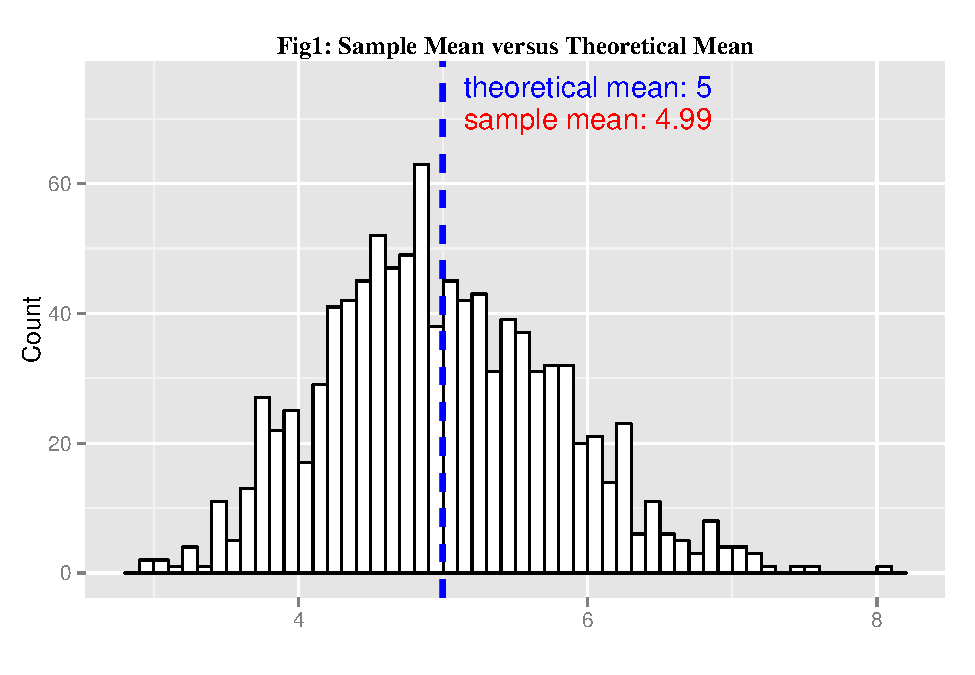
\includegraphics{PA1pdf_files/figure-latex/unnamed-chunk-3-1.pdf}

Plot the histogram of a thousand of simulated variances and compare the
average of these variances with its theoretical value.

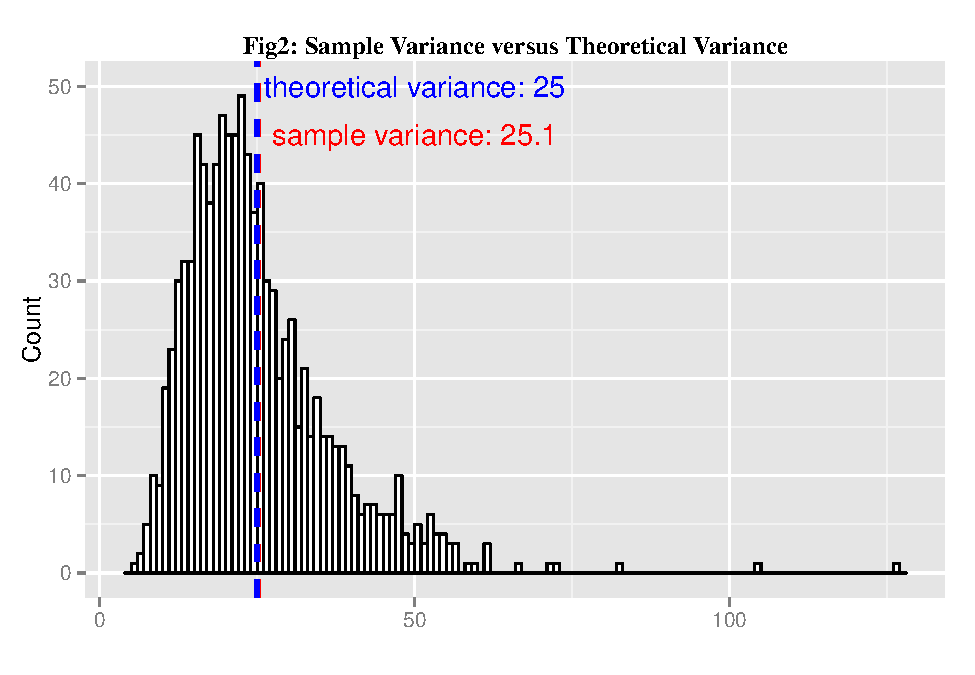
\includegraphics{PA1pdf_files/figure-latex/unnamed-chunk-5-1.pdf}

\subsubsection{Comparison with the Central Limit
Theorem}\label{comparison-with-the-central-limit-theorem}

The \textbf{law of large numbers (LLN)} states that the average of the
results obtained from a large number of trials should be close to the
expected value. As shown in both \texttt{Fig1} and \texttt{Fig2}, mean
and variance are close to their theoretical values. Futher more, the
\texttt{Central\ Limit\ Theorem} (CLT) states that the distribution of
averages of iid variables, properly normalized, becomes that of a
standard normal as the sample size increases.

\paragraph{Nomarlization}\label{nomarlization}

Here we normalize both sample mean and variance and compare with the
standard normal distribution.

Now plot both distributions of sample mean and variance and overlay with
the standard normal distribution.

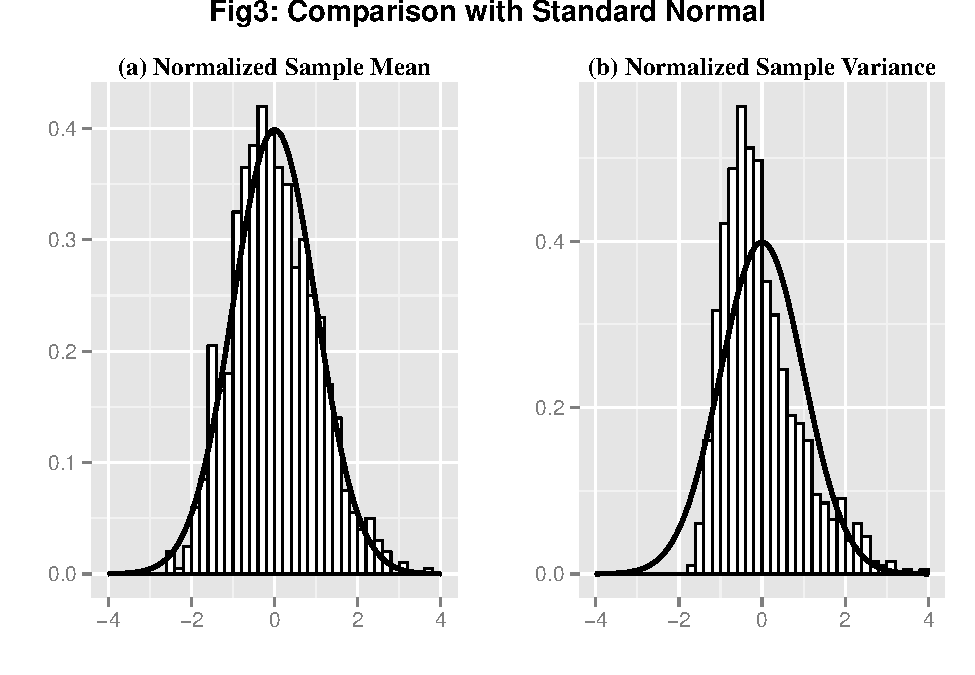
\includegraphics{PA1pdf_files/figure-latex/unnamed-chunk-7-1.pdf}

As we can see in \texttt{Fig3}, both \texttt{(a)} and \texttt{(b)} are
close to standard normal distribution, which center at 0 and most of the
data are within 3 times \(\sigma\). But variance distribution is more
skewing to the right. This might due to the limitation of the CLT that
doesn't give the exact sample size.

\end{document}
